\section{動的シナプス}

シナプス前活動に応じて\textbf{シナプス伝達効率}\index{しなぷすでんたつこうりつ@シナプス伝達効率} (synaptic efficacy)が動的に変化する性質を\textbf{短期的シナプス可塑性}\index{たんきてきしなぷすかそせい@短期的シナプス可塑性} (Short-term synaptic plasticity)といい,このような性質を持つシナプスを\textbf{動的シナプス}\index{どうてきしなぷす@動的シナプス} (dynamical synapses)と呼ぶ.シナプス伝達効率が減衰する現象を短期抑圧 (short-term depression; STD),増強する現象を短期促通(short-term facilitation; STF)という.さらにそれぞれに対応するシナプスを減衰シナプス,増強シナプスという.

ここでは\cite{Mongillo2008-kk}および\cite{Orhan2019-rq}で用いられている定式化を使用する.


\begin{gathered}
\frac{\mathrm{d} x(t)}{\mathrm{d} t}=\frac{1-x(t)}{\tau_{x}}-u(t) x(t) r(t) \Delta t \\
\frac{\mathrm{d} u(t)}{\mathrm{d} t}=\frac{U-u(t)}{\tau_{u}}+U(1-u(t)) r(t) \Delta t
\end{gathered}


ただし,定数は以下のようにする.
\begin{itemize}
\item STSP neurotransmitter time constant: $\tau_x$ 200 ms/1,500 ms (facilitating/depressing)
\item STSP neurotransmitter utilization: $\tau_u$ 1,500 ms/200 ms (facilitating/depressing)
\item STSP neurotransmitter increment: $U$ 0.15/0.45 (facilitating/depressing)
\item Time step (training and testing): $\Delta t$ 10ms
\end{itemize}

\begin{itemize}
\item $x$: the fraction of available neurotransmitter
\item $u$: the neurotransmitter utilization
\end{itemize}
\lstinputlisting[language=julia]{./text/synapse-model/dynamical-synapses/001.jl}
\lstinputlisting[language=julia]{./text/synapse-model/dynamical-synapses/002.jl}
\lstinputlisting[language=julia]{./text/synapse-model/dynamical-synapses/003.jl}
\lstinputlisting[language=julia]{./text/synapse-model/dynamical-synapses/004.jl}
\lstinputlisting[language=julia]{./text/synapse-model/dynamical-synapses/005.jl}
\begin{figure}[ht]
	\centering
	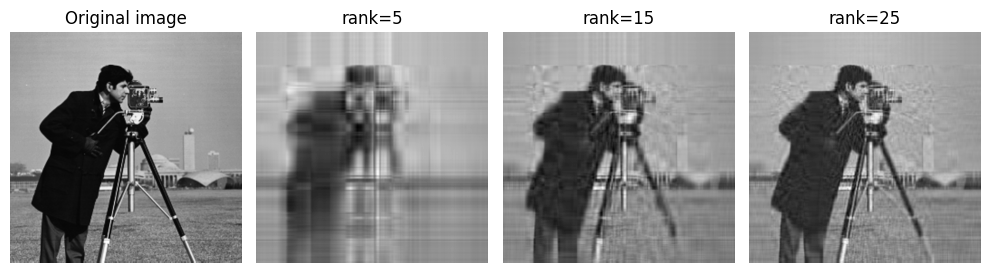
\includegraphics[scale=0.8, max width=\linewidth]{./fig/solve-credit-assignment-problem/linear-network-learning-dynamics/cell005.png}
	\caption{cell005.png}
	\label{cell005.png}
\end{figure}
